\cotefile{132}
\scanpage{19}
% upper diagram and its branches
\diagram{\begin{tikzcd}[ampersand replacement=\&,row sep=1.2em,column sep=.65em]
\& \mathrm{SO} \& \& \& \\
\& \& \mathrm{PLO}\arrow[ul]\arrow[dl,""{name=pl,coordinate}]\arrow[drr,""{name=pr,coordinate}] \& \& \\
\text{clair} \& \unsure{\mathrm{TUBo}|\mathrm{TUB0}|\mathrm{TUBO}}\arrow[dl,"{\unsure{\simeq|\approx}}"']\arrow[dr,""{name=ts,coordinate}] \& \& \& \mathrm{SOB}\arrow[dl,"{-\partial\;(\simeq\partial)}"]\\
\unsure{\mathrm{Rec}|\mathrm{Rcc}|\mathrm{Kc}} \& \& \mathrm{SOB}\arrow[r,"\partial"] \& \mathrm{CO} \& \\
\& \& \& \rotatebox{90}{$\simeq$} \& \\
\& \& \& \unsure{\mathrm{Ens}\,f|\mathrm{Ensf}|\mathrm{Equiv}} \& \\
\& \& \& (\mathbb{N},\{\unsure{\mathfrak{S}_n|\mathcal{S}_n|\mathfrak{G}_n}\}) \& \text{comme,}\\
\& \& \text{il suffit de les déterminer} \& \&
\arrow[from=pl,to=3-1,bend right=18,thin]
\arrow[from=pr,to=7-5,bend left=10,thin]
\arrow[from=ts,to=8-3,bend right=56,thin]
\end{tikzcd}}

% brace to the right of PLO, upper then lower member
\[\left\{\begin{aligned}
 &\text{complexes \unsure{hypercirculoïdisés|hypercircularisés|hypercirculoïsés|hypercirculaires} (i.e.\ 1-complexes \deleted{\unsure{dont}} circuloïdisés \(K\)}\\
 &\quad\text{avec une partie \(\Pi'\) de \(\mathrm{Circ}(K)\) (ens.\ des circuits)) et}\\
 &\quad\text{application \(\pi'\xrightarrow{g}\mathbb{N}\).}\\
 &\text{extensions des groupes de symétries de 1-complexes \unsure{combinat.|combinatoires}}\\[-2pt]
 &\quad\text{hypercirculoïdisés \deleted{\unsure{hyperboliques}}\inserted{spéciaux} par des groupes de Teichmüller.}
\end{aligned}\right.\]

% below PLO / along the two outgoing arrows
(car \(\pi_0(K)\to\pi_0(S)\)) surjectif \deleted{\unsure{\(g\)}}

% upper right
\(\prod_i T'_{g_i,n_i}\) ; ces ext. sont connues quand on connaît les \(T'_{g_i,n_i}\) séparément, \deleted{\unsure{et}} les hom. canoniques
\[
 \mathbb{Z}^{n_i}\unsure{\lhook\joinrel\to|\to|\xrightarrow{\lambda}}\mathrm{Centre}(L_{g_i,n_i})
\]
et les ext. de Ladegaillerie.
\[
 1\longrightarrow T'_{g_i,n_i}\longrightarrow L_{g_i,n_i}
 \longrightarrow\mathfrak{S}_{\deleted{\unsure{k}}n_i}\longrightarrow1
\]

\margin{cf ci-contre}

% left, beneath Rec
\margin{\(\Leftrightarrow\) [1-complexes combinatoires circuloïdisés] pr. \unsure{quelles|quels} les classes d'isomorphie de 1-complexes circuloïdisés connexes, groupes de symétries des complexes circuloïdisés : doit se ramener à la détermination des groupes de symétries des \unsure{sous-complexes 1-circulaires|sous-complexes 1-circularisés|1-complexes circulaires} connexes}

% middle beneath the left SOB
(familles finies de couples \((g_i,n_i)\)) (genre, nb de trous) \(g\geq0,\ n\geq0\) ; ``groupes de Teichmüller à trous'' ; ou : familles finies de groupes extérieurs à lacets

Tout se détermine \unsure{à|:|: à} l'aide des ``gr. de Teichmüller à trous'' ordinaires \(T_{g,n}\)

% right; fine line from the sloping branch. The framed lines are hatched out
\deleted{\unsure{groupes des auto}\inserted{en termes des} \unsure{groupements} \unsure{disant que}
\(L_{g_i,n_i}\unsure{\times|\twoheadrightarrow|\to}T_{h_i,n_i}\simeq L_{g_i,n_i}/\unsure{\mathrm{Im}}({\unsure{\mathbb{Z}}}^{n_i})\)
de noyau \(\mathrm{Im}(\mathbb{Z}^{n_i}\to L_{g_i,n_i})\)}
ce qui est dit dessus

% bottom; fine line from TUBo--SOB
pour les \deleted{\unsure{des}} \unsure{ordinaires|cas} connexes i.e les 1-compl. circ connexes.

Le calcul de \(g,n\) est donné par Yves Il reste, pour un tel \(K\) \deleted{\unsure{déterminer}} de déterminer
\[
 \boxed{\mathrm{Aut}_{\mathrm{circ}}(K)_{\deleted{\unsure{0|*}}}
 \longrightarrow\mathrm{Aut}(\unsure{\mathrm{Tub}(K)|\mathrm{Tub}\lvert K\rvert})\simeq T_{g,n}}
\]
% archive sheet number: 18

\scanpage{20}
\textcircled{B}
Supposons à la fois
\[
\begin{aligned}
\alpha)&\quad \widetilde H_0\ \text{est connexe et simplement connexe}\\
\beta)&\quad \pi\subset\widetilde H_0\\
\gamma)&\quad \pi,N,\unsure{\mathfrak{S}|\mathcal{G}|\mathfrak{G}}\ \text{discret}
\end{aligned}
\]
Comme \(\mathfrak{S}\) discret, \(\widetilde H_0\) connexe, on a
\[
\boxed{\left\{\begin{aligned}
\widetilde H_0&=\widetilde H^{0}\quad\text{(composante neutre)}\\
\mathfrak{S}&=\pi_0\widetilde H
\end{aligned}\right.}
\]
Comme \(\pi\subset\widetilde H_0\), on a que \(H=\widetilde H/\pi\) est une extension de \(\mathfrak{S}\) par \(H^0=\widetilde H_0/\pi\)
\[
\boxed{H^0=\widetilde H_0/\pi,\quad \mathfrak{S}=\pi_0(H)}
\]
Comme \(\widetilde H_0\) est simplement connexe, \deleted{c'est le}\inserted{\(\pi\) discret, \(\widetilde H_0\) est} le revêtement universel de \(H^0=\widetilde H_0/\pi\)
\[
\boxed{\left\{\begin{aligned}
\widetilde H^{0}&=\text{rev. universel de }H^0\\
\pi&=\pi_1(H^0)=\pi_1(H)
\end{aligned}\right.}
\]
Donc la situation équivaut :

\(1^\circ)\) donnée d'un groupe top \(H\), \deleted{\unsure{entre}}\unsure{q|i.e.} [qui est donc ext. d'un grpe discret \(\mathfrak{S}=\pi_0(H)\) par \deleted{\unsure{l'un}} groupe connexe \(H^0\)] ; ce dernier \deleted{\unsure{\(2^\circ)\)}} a un groupe \unsure{revêtmt|revêtant} universel \(\widetilde H^0\), extension de \(H^0\) par \(\pi\simeq\pi_1(H^0)\)]
\margin{groupe \uuline{comm.} sur lequel \(\mathfrak{S}\) opère}

\(2^\circ)\) Une extension \(\widetilde H\) de \(H\) par \(\pi\) qui prolonge l'extension \(\widetilde H^0\) de \(H^0\) par \(\pi=\pi_1(H^0)\)

\uline{NB} Une telle extension n'est pas nécessairement unique à isom près ; elle est unique modulo une extension de \(\mathfrak{S}\) par \(\pi\), \inserted{i.e. mod. \unsure{éltmt|élémt|action} de \(H^2(\mathfrak{S},\pi)\),} et sauf erreur l'obstruction à l'existence d'une telle ext. est dans \(H^3(\mathfrak{S},\pi)\). Une telle extension existe si \(H\) est produit semi direct \(\mathfrak{S}.H^0\), car on peut prendre alors \(\widetilde H=\mathfrak{S}.\widetilde H^0\).

% slanted
\margin{\uline{NB} \(G_0=\pi_0\widetilde G=\widetilde G/\widetilde G^0\) (\(\widetilde G^0\to\widetilde H^0\) est un isom) \deleted{\unsure{en termes de}} et comme \(G=\widetilde G/\pi\), on trouve que}
% slanted; same marginal note, branches below its horizontal sequence
\diagram{\begin{tikzcd}[ampersand replacement=\&,column sep=1.2em,row sep=.65em]
\pi\arrow[r]\arrow[dddr] \& \pi_0\widetilde G\arrow[r]\arrow[d,equal] \& \pi_0G\arrow[r] \& 1\\
\&G_0\arrow[d,phantom,"{\cup}"]\&\&\\
\&N\arrow[d,phantom,"{\cup}"]\&\&\\
\&\mathfrak{z}(N)\&\&
\end{tikzcd}}

\(3^\circ)\) Le groupe discret \(N\)

Avec ces données, on trouve que \uline{la catégorie des extensions de \(H\) par \(N\)} équivaut à celle des couples \((\deleted{\unsure{H}}G_0,\varphi)\), où \(\deleted{\unsure{H}}G_0\) est une ext. de \(\mathfrak{S}\) par \(N\) et \(\varphi:\pi\longrightarrow\mathfrak{z}(N)^{\mathfrak{S}}\) un hom \((\mathfrak{z}(N)=\text{centre de }N)\)
% archive sheet number: 19

\scanpage{21}
On peut aussi expliciter ainsi la construction de l'extension \(G\) \inserted{de \(H\) par \(N\)} associée à l'ext \(\deleted{\unsure{H}}G_0\) de \(\unsure{\mathfrak{S}|\mathcal{G}|\mathfrak{G}}\) par \(N\) et le \(\mathfrak{S}\)-hom \(\varphi:\deleted{\unsure{\mathfrak{S}}}\pi\to\mathfrak{z}(N)\) :

Soit \(G_{!}^{\deleted{\unsure{\xi|\varphi}}}\) l'ext. de \(H\) par \(N\) image inverse de l'ex \(G_0\) (de \(\mathfrak{S}\) par \(N\)) via \(H\to\mathfrak{S}\). Considérons l'extension \(\widetilde H\) de \(H\) par \(\pi\), \unsure{lé|le} \(\mathfrak{S}\)-hom \(\varphi:\pi\to\mathfrak{z}(N)\) nous donne une extn \unsure{corresp.|centrale} \(\widetilde H^{\varphi}_{\deleted{\unsure{\xi|\ast}}}\) de \(H\) par \(\mathfrak{z}(N)\), correspondant aux \(=\) opérations de \(H\) (et \(\mathfrak{S}\)) sur \(\mathfrak{z}(N)\) que l'ext. \(G_1\). On peut donc prendre le produit contracté des deux \inserted{extensions} \(G_1\) et \(\widetilde H^\varphi\), on trouve le \(G\) cherché.

D'ailleurs, \deleted{\unsure{soit}} comme \(G\) est un \unsure{revêtmt|revêtement} de \(H\), on aura
\[
 \pi_i(G)\xrightarrow{\sim}\pi_i(H)\quad\text{si }i\geq2
\]
\margin{\unsure{\(1\)}}
\diagram{\begin{tikzcd}[ampersand replacement=\&,column sep=.45em,row sep=.55em]
\pi_1(G)=\mathrm{Ker}\bigl( \& \pi_1(H)\arrow[r]\arrow[d,equal] \& \pi_0(N)\arrow[d,equal] \& \bigr)\\
\& \pi\arrow[r]\arrow[dr,"\varphi"'] \& N\arrow[d,phantom,"\rotatebox{90}{$\subset$}"] \&\\
\& \&\mathfrak{z}(N)\&
\end{tikzcd}}
\diagram{\begin{tikzcd}[ampersand replacement=\&,column sep=1em,row sep=.6em]
\pi_1(H)\arrow[r]\arrow[d,equal] \& N\arrow[r]\arrow[d,phantom,"\rotatebox{90}{$\subset$}"] \& \pi_0(G)\arrow[r]\&\pi_0(H)\arrow[r]\arrow[d,equal]\&1\\
\pi\arrow[r,"\varphi"']\&\mathfrak{z}(N)\&\&\mathfrak{S}\&
\end{tikzcd}}
\margin{i.e. \(\pi_0G\) est une \unsure{ext.|cat.} de \(\mathfrak{S}\) par \(\mathrm{Coker}(\varphi:\pi\to N)\)}

et on vérifie que l'on a une suite exacte
\[
 \deleted{\pi_0(\unsure{G})=}\qquad
 \pi\longrightarrow G_0\longrightarrow\pi_0(G)\longrightarrow1
\]
\[
 \deleted{\pi_0(G)\to G_0(\unsure{\mathfrak{S}})}
\]
(i.e. \(\pi_0(G)=\mathrm{Coker}(\pi\to G_0)\)) où

\(\pi\to G_0\) est le composé
\[
 \pi\longrightarrow\mathfrak{z}(N)\lhook\joinrel\longrightarrow N\lhook\joinrel\longrightarrow G_0\qquad \ldots\,..
\]

\textcircled{\(B'\)} Supposons seulement \(\pi,N,H\) discrets, \(\pi\subset\widetilde H_0\) (conditions \(\beta)\) et \(\gamma)\) mais pas néc. \(\alpha)\) (i.e. que \(\widetilde H_0\) soit connexe ou simplement connexe).

\(N\) étant discret, on a encore
\[
 \pi_i(G)\xrightarrow{\sim}\pi_i(H)\quad\text{si }i\geq2
\]
\hfill TSVP
% archive sheet number: 20

\scanpage{22}
\diagram{\begin{tikzcd}[ampersand replacement=\&,column sep=1em,row sep=.7em]
\pi_1G=\mathrm{Ker}\,( \& \pi_1(H)\arrow[r,""{name=k,coordinate}]\arrow[dd,""{name=v,coordinate}] \& \pi_0N\arrow[d,equal] \\
\phantom{\partial} \& \& N\arrow[d,phantom,"{\cup}"]\\
\& \pi_0(\pi)=\pi\arrow[ur]\arrow[r,"\varphi"'] \& \mathfrak{z}(N)
\arrow[from=1-2,to=k,phantom,shift left=2ex,"{\text{(connu)}\downarrow}"]
\arrow[from=v,to=2-1,no head,thin,bend right=12,shorten >=1.5em]
\arrow[from=3-2,to=3-3,no head,thin,start anchor=south,end anchor=south,bend right=66,shorten >=.7em]
\end{tikzcd}}
\margin{[\(\partial\) associé à suite exacte d'homotopie pour ext. \(1\to\pi\to\widetilde H\to H\to1\)]}
\margin{Car \(\pi\) discret}

\deleted{\unsure{et}} et on a
\diagram{\begin{tikzcd}[ampersand replacement=\&,column sep=1.1em,row sep=1em]
\pi_1H\arrow[r,"{\text{connu}\,\downarrow}"]\arrow[d,"\partial"'] \& N\arrow[r] \& \pi_0G\arrow[r] \& \pi_0H\arrow[r]\&1\\
\pi\arrow[r,"\varphi"] \& \mathfrak{z}(N)\arrow[u,hook] \& \&\&
\end{tikzcd}}
i.e. \(\pi_0G\deleted{\unsure{{}_0}}\) est une extension de \(\pi_0H\) par \(\mathrm{Coker}\,(\pi_1H\to N]\). Or on a une extension \(G_0\) de \(\unsure{\mathfrak{S}|\mathcal{G}|\mathfrak{G}}\) par \(N\) d'où, grâce à \(H\to\mathfrak{S}\) \inserted{(défini car \(\pi\subset\widetilde H_0\))} (i.e. \(\pi_0H\to\mathfrak{S}\) (\(=\pi_0\mathfrak{S}\)) car \(\mathfrak{S}\) discret) une extension \(G_1\) de \(\pi_0H\) par \(\deleted{\mathfrak{S}}N\) ;

% slanted
\margin{\rotatebox{30}{faux}\quad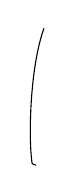
\begin{tikzpicture}[baseline]\draw[thin] (0,.6) .. controls (-.18,.1) and (-.20,-.8) .. (-.15,-1.12) -- (-.10,-1.14);\end{tikzpicture}}
On vérifie alors qu'on a
\diagram{\begin{tikzcd}[ampersand replacement=\&,column sep=.65em,row sep=.6em]
\pi_0G\simeq\mathrm{Coker}\,( \& \pi_1H\arrow[r]\arrow[dd,"\partial"] \& G_1\arrow[d,phantom,"\cup"]\& )\\
\& \& N\arrow[d,phantom,"\cup"]\&\\
\& \pi\arrow[r,"\varphi"] \&\mathfrak{z}(N)\&
\end{tikzcd}}
% archive sheet number: 21

\scanpage{23}
\deleted{\textcircled{D}} \textcircled{C} Soit, sous les conditions de \textcircled{A},
\[
 H'\xrightarrow{u}H
\]
un hom de groupes topologiques. On en déduit par image inverse une extension
\diagram{\begin{tikzcd}[ampersand replacement=\&,column sep=1em]
(b')\&1\arrow[r]\&\pi\arrow[r]\arrow[d,equal]\&\widetilde H'\arrow[r]\arrow[d]\&H'\arrow[r]\arrow[d,"u"]\&1\\
(b\&1\arrow[r]\&\pi\arrow[r]\&\widetilde H\arrow[r]\&H\arrow[r]\&1
\end{tikzcd}}
et désignant par \(\widetilde H'_0\) l'image inverse de \(\widetilde H_0\) par \(\widetilde H'\to\widetilde H\), on trouve, posant \(\unsure{\mathfrak{S}'|\mathcal{G}'|\mathfrak{G}'}=\widetilde H'/\widetilde H'_0\lhook\joinrel\to\mathfrak{S}\), une suite exacte
\diagram{\begin{tikzcd}[ampersand replacement=\&,column sep=1em]
(a')\&1\arrow[r]\&\deleted{\unsure{\pi|\widetilde H}}\widetilde H'_0\arrow[r]\arrow[d]\&\widetilde H'\arrow[r]\arrow[d]\&\mathfrak{S}'\arrow[r]\arrow[d,hook]\&1\\
(c)\&1\arrow[r]\&\widetilde H_0\arrow[r]\&\widetilde H\arrow[r]\&\mathfrak{S}\arrow[r]\&1
\end{tikzcd}}

Considérons maintenant \deleted{\unsure{la}} l'extension \(G'\) de \(H'\) par \(N\) image inverse de \(G\) par \(H'\to H\)
\diagram{\begin{tikzcd}[ampersand replacement=\&,column sep=1em]
(\unsure{e|c|{-}}')\&1\arrow[r]\&N\arrow[r]\arrow[d,Rightarrow]\&G'\arrow[r]\arrow[d]\&H'\arrow[r]\arrow[d]\&1\\
(e)\&1\arrow[r,phantom,"{\unsure{{-}|\to}}" description]\&N\arrow[r,no head]\&G\arrow[r,no head]\&H\arrow[r,no head]\&1
\end{tikzcd}}
, son image inverse par
\diagram{\begin{tikzcd}[ampersand replacement=\&,column sep=2em,row sep=.8em]
\widetilde H'_0\arrow[r]\arrow[d,dotted]\&H'\arrow[d,dashed]\\
\widetilde H_0\arrow[r,dashed]\&H
\end{tikzcd}}
est munie de façon évidente d'une trivialisation stricte, \deleted{\unsure{donc}} (grâce à celle de l'image inverse de \(G\) par \(\widetilde H_0\to H\)) donc elle est déterminée par

\(1^\circ)\) une ext. \(\widetilde G'_0\) \deleted{de} \(\mathfrak{S}'\) par \(N\)
\[
 1\longrightarrow N\longrightarrow \widetilde G'_0\longrightarrow\mathfrak{S}'\longrightarrow1
\]
% archive sheet number: 22

\scanpage{24}
\(2^\circ)\) Un hom \(\pi\xrightarrow{\varphi'}\widetilde G'_0\) qui centralise \(N\) et remonte \(\pi\to\unsure{\mathfrak{S}'|\mathcal{G}'|\mathfrak{G}'}\) [donc, si \(\pi\subset\widetilde H_0\) d'où \(\deleted{\pi\to}\pi\to\mathfrak{S}'\lhook\joinrel\to\mathfrak{S}\) trivial, un hom
\[
 \pi\xrightarrow{\varphi'}\mathfrak{z}(N)\qquad ]
\]

Ceci posé, on vérifie immédiatement que l'extension \(\widetilde G'_0\) est l'image inverse de \(\widetilde G_0\) par \(\mathfrak{S}'\to\mathfrak{S}\), \deleted{et que} (donc \(\widetilde G'_0\subset\widetilde G_0\)), et que \(\varphi'\) est induit par \(\varphi\) [donc si \(\pi\subset\widetilde H_0\), \(\varphi=\varphi'\) en tant que hom \(\pi\to\mathfrak{z}(N)\)]

Si les conditions \deleted{\unsure{\(\alpha)\)}} \(\beta)\ \gamma)\) sont \unsure{vérifiées|vérifiés} pour les données \deleted{\unsure{\(a)\)}}\inserted{\(a)\)} \(b)\ \unsure{e|c})\), il en est de \(=\) pour les données \deleted{\unsure{\(a)\ b)\ e)\)}} \(a')\,b')\,e')\) (\(\pi,N,\mathfrak{S}'\) discrets, \(\pi\subset\widetilde H'_0\)) mais la condition \(\alpha\) (\(\widetilde H_0^{\deleted{\unsure{0|\prime|\ast}}}\) connexe et simplement connexe n'implique pas néc. \(=\) que \(\widetilde H'_0{}^{\deleted{\unsure{0}}}\) soit connexe \ldots)

\deleted{Mais comme \(\mathfrak{S}'\) est discret, \(\deleted{\unsure{\widetilde H'_0}}\), il en est de \(=\) de \(G'_0\), donc \(G'_0\) apparaît comme un quotient de \(\pi_0\widetilde G'\)}
% archive sheet number: 23

\scanpage{26}
\textbf{C. R. Acad. Sc. Paris, t. 279 (22 juillet 1974)}\hfill\textbf{Série A ---}\mspage{129}\par\noindent\rule{\linewidth}{.35pt}\par

TOPOLOGIE. --- \textit{Classification topologique des plongements des 1-complexes compacts dans les surfaces.} Note (*) de M. \textbf{Yves Ladegaillerie}, présentée par M. Henri Cartan.

{\small On établit l'équivalence de la catégorie isotopique des voisinages tubulaires orientés des 1-complexes avec la catégorie des 1-complexes circularisés. On établit ensuite l'équivalence de la catégorie isotopique des voisinages tubulaires quelconques des 1-complexes avec la catégorie des 1-complexes munis d'un automorphisme involutif sans point fixe et d'une circularisation antisymétrique. Enfin on caractérise les plongements dans des surfaces orientées de genre minimal.}

7. \textsc{Voisinages tubulaires des 1-complexes.} --- La terminologie et les notations sont celles de (\textsuperscript{1}). Dans la suite \(\mathrm{K}\) désigne un 1-complexe topologique compact.

7.1. \textsc{Théorème.} --- \textit{Soit \(i\) un plongement de \(\mathrm{K}\) connexe dans une surface à bord compacte orientée \(\mathrm{X}\), soit \(\mathrm{A}\) un anneau non réduit à \(0\). Il y a équivalence entre :}

\textit{(a) \(i\) est une équivalence d'homotopie ;}

\textit{(b) \(i\) est équivalent à un plongement standard \(i_\omega\) [cf.} (\textsuperscript{1}), 3.3] ;

\textit{(c) \(x\mathrel{\ooalign{\hfil$\simeq$\hfil\cr\hfil$\vert$\hfil\cr}}\mathrm{S}^2\), \(\pi_0(i)\) \textup{et} \(\pi_1(i)\) sont des isomorphismes ;}

\textit{(d) \(\mathrm{X}\mathrel{\ooalign{\hfil$\simeq$\hfil\cr\hfil$\vert$\hfil\cr}}\mathrm{S}^2\), \(\mathrm{X}\) connexe et \(\mathrm{H}_1(i)\) est un isomorphisme de \(\mathrm{H}_1(\mathrm{K}\,;\mathrm{A})\) sur \(\mathrm{H}_1(\mathrm{X}\,;\mathrm{A})\) ;}

\textit{(e) \(\mathrm{X}\mathrel{\ooalign{\hfil$\simeq$\hfil\cr\hfil$\vert$\hfil\cr}}\mathrm{S}^2\), \(\mathrm{X}\) connexe et \(\mathrm{H}^1(i)\) est un isomorphisme de \(\mathrm{H}^1(\mathrm{K}\,;\mathrm{A})\) sur \(\mathrm{H}^1(\mathrm{X}\,;\mathrm{A})\).}

On dira alors que \((\mathrm{X},i)\) est un \textit{voisinage tubulaire orienté de} \(\mathrm{K}\).

7.2. Plus généralement on appelle \textit{voisinage tubulaire} d'un 1-complexe \(\mathrm{K}\) tout couple \((\mathrm{X},i)\) où \(i\) est un plongement de \(\mathrm{K}\) dans la surface compacte à bord \(\mathrm{X}\) et \(i\) est une équivalence d'homotopie. Ce sont les objets de la \textit{catégorie isotopique des voisinages tubulaires} notée TUB, un \textit{morphisme entre les voisinages tubulaires} \((\mathrm{X},i)\) et \((\mathrm{X}',i')\) de \(\mathrm{K}\) et \(\mathrm{K}'\) étant une classe d'isotopie d'homéomorphismes \(h\) de \(\mathrm{X}\) sur \(\mathrm{X}'\) tel\unsure{\textperiodcentered|.} que \(h(i(\mathrm{K}))=i'(\mathrm{K}')\).

7.3. La \textit{catégorie isotopique des voisinages tubulaires orientés} est la catégorie TUBO dont les objets sont les voisinages tubulaires orientés de 1-complexes et dont les morphismes sont les morphismes de voisinages tubulaires qui respectent l'orientation.

8. \textsc{La catégorie isotopique des 1-complexes circularisés.}

8.1. C'est la catégorie \(\mathrm{K}\,\omega_{\mathrm{I}}\) dont les objets sont les couples \((\mathrm{K},\omega)\) où \(\mathrm{K}\) est un 1-complexe quelconque et \(\omega\) une circulation de \(\mathrm{K}\). Un morphisme de \((\mathrm{K},\omega)\) dans \((\mathrm{K}',\omega')\) est une classe d'isotopie d'homéomorphismes de \(\mathrm{K}\) dans \(\mathrm{K}'\) qui respecte la circulation.

8.2. On a un foncteur \(\mathrm{T}\) de \(\mathrm{K}\,\omega_{\mathrm{I}}\) dans TUBO qui à \((\mathrm{K},\omega)\) associe le voisinage tubulaire standard \(\mathrm{T}(\mathrm{K},\omega)\) (\textsuperscript{1}) et qui à un morphisme \(\bar h:(\mathrm{K},\omega)\to(\mathrm{K}',\omega')\) associe le morphisme \(\mathrm{T}(\bar h)\) de voisinages tubulaires classe de l'homéomorphisme \(\mathrm{H}:\mathrm{T}(\mathrm{K},\omega)\to\mathrm{T}(\mathrm{K}',\omega')\) défini à partir des homéomorphismes \(\mathrm{H}_a:\bar a\times\mathrm{I}\to\unsure{\overline{h(a})|\overline{h(a)}}\times\mathrm{I}\) (\(a\) étant un arc de \(\mathrm{K}\)) qui à \((x,t)\) associe \((h(x),t)\).

% right margin of 8.2, a shallow curved pen stroke and two dots
\figure{\begin{tikzpicture}[x=1cm,y=1cm]\draw[thin] (0,0) .. controls (.44,-.12) and (.93,-.18) .. (1.05,.04);\fill (.32,.37) circle (.012);\fill (.39,.44) circle (.008);\end{tikzpicture}}

8.3. \textsc{Théorème.} --- \textit{\(\mathrm{T}\) est une équivalence entre les catégories \(\mathrm{K}\,\omega_{\mathrm{I}}\) et TUBO.}

9. \textsc{La catégorie isotopique des \(\mathbf{Z}_2\)-voisinages tubulaires orientés.}

9.1. C'est la catégorie \(\widetilde{\mathrm{TUBO}}\) dont les objets sont les couples \((\widetilde{\mathrm{T}},\theta)\) où \(\widetilde{\mathrm{T}}\) est un objet de TUBO et \(\theta\) un homéomorphisme de voisinage tubulaire de \(\widetilde{\mathrm{T}}\) sur \(\widetilde{\mathrm{T}}\), involutif, sans
% archive sheet number: 25

\scanpage{27}
\mspage{130}\textbf{--- Série A}\hfill\textbf{C. R. Acad. Sc. Paris, t. 279 (22 juillet 1974)}\par\noindent\rule{\linewidth}{.35pt}\par

point fixe et qui inverse l'orientation. Un morphisme entre \((\widetilde{\mathrm{T}},\theta)\) et \((\widetilde{\mathrm{T}}',\theta')\) est une classe d'isotopie \(\bar h\) d'homéomorphisme \(h\) de voisinages tubulaires de \(\widetilde{\mathrm{T}}\) sur \(\widetilde{\mathrm{T}}'\) tel que \(h\,\theta=\theta'\,h\).

9.2. On définit un foncteur \(\mathrm{Q}\) de \(\widetilde{\mathrm{TUBO}}\) dans TUB qui à un objet \((\widetilde{\mathrm{T}},\theta)\) de \(\widetilde{\mathrm{TUBO}}\) associe le voisinage tubulaire quotient de \(\widetilde{\mathrm{T}}\) par \(\theta\) et qui à un morphisme associe le morphisme quotient.

9.3. \textsc{Proposition.} --- \textit{\(\mathrm{Q}\) est une équivalence entre les catégories \(\widetilde{\mathit{TUBO}}\) et TUB.}

10. \textsc{La catégorie isotopique des \(\mathbf{Z}_2\)-1-complexes circularisés.}

10.1. C'est la catégorie \(\widetilde{\mathrm{K}}\,\omega_{\mathrm{I}}\) dont les objets sont les triplés \((\widetilde{\mathrm{K}},\widetilde\omega,\theta)\) où \((\widetilde{\mathrm{K}},\widetilde\omega)\) est un objet de \(\mathrm{K}\,\omega_{\mathrm{I}}\) et \(\theta\) un homéomorphisme involutif sans point fixe de \(\widetilde{\mathrm{K}}\) qui inverse la circularisation (on dira que \(\widetilde\omega\) est \textit{antisymétrique}). Un morphisme entre \((\widetilde{\mathrm{K}},\widetilde\omega,\theta)\) et \((\widetilde{\mathrm{K}}',\widetilde\omega',\theta')\) est une classe d'isotopie \(\bar h\) d'homéomorphisme \(h\) de \(\widetilde{\mathrm{K}}\) sur \(\widetilde{\mathrm{K}}'\) qui respecte les circularisations et tel que \(h\,\theta=\theta'\,h\).

10.2. Le foncteur \(\mathrm{T}\) induit un foncteur \(\widetilde{\mathrm{T}}\) de \(\widetilde{\mathrm{K}}\,\omega_{\mathrm{I}}\) dans \(\widetilde{\mathrm{TUBO}}\).

\textsc{Théorème.} --- \textit{\(\widetilde{\mathrm{T}}\) est une équivalence de catégories entre \(\widetilde{\mathrm{K}}\,\omega_{\mathrm{I}}\) et \(\widetilde{\mathit{TUBO}}\).}

\textsc{Corollaire.} --- \textit{Les catégories \(\widetilde{\mathrm{K}}\,\omega_{\mathrm{I}}\) et TUB sont équivalentes.}

11. \textsc{La catégorie isotopique des 1-complexes cocircularisés.}

11.1. Une \textit{cochaîne} sur \(\mathrm{K}\) est une application \(\gamma\) de \(\mathrm{A}\) (arcs de \(\mathrm{K}\)) dans \(\mathbf{Z}_2\) (i. e. \(\mathbf{Z}/2\,\mathbf{Z}\)) telle que \(\gamma\sigma=\gamma\) [\textit{voir} (\textsuperscript{1})]. Si \(\omega\) et \(\omega'\) sont deux circularisations de \(\mathrm{K}\) telles que pour tout sommet \(s\) de degré \(\geqq3\) (le degré \(\mathring{d}s\) de \(s\) est le nombre d'arcs issus de \(s\)) \(\omega_s\) et \(\omega'_s\) soient égaux ou inverses l'un de l'autre (ce qu'on notera \(\lvert\omega_s\rvert=\lvert\omega'_s\rvert\)), on désigne par \(\omega'_s/\omega_s\) leur « rapport » qui vaut \(1\) dans le premier cas, \(-1\) dans le second. Si on note \(\varphi\) l'isomorphisme du groupe multiplicatif \(\{-1,1\}\) dans \(\mathbf{Z}_2\), on définit un « cobord » \(\chi_{\omega\omega'}\), application définie sur l'ensemble des arcs qui n'ont pas d'extrémités de degré 1, qui à un arc d'extrémités \(s_0\) et \(s_1\) associe \(\varphi\,(\omega'_{s_1}/\omega_{s_1})-\varphi\,(\omega'_{s_0}/\omega'_{s_0})\), et qui à une boucle isolée associe \(0\).

11.2. \(\mathrm{K}\) étant donné, on définit une relation d'équivalence sur les couples \((\gamma,\omega)\) où \(\gamma\) est une cochaîne, \(\omega\) une circularisation par \((\gamma,\omega)\sim(\gamma',\omega')\Leftrightarrow\) pour tout sommet \(s\) de \(\mathrm{K}\) tel que \(\mathring d s\geqq3\) on a \(\lvert\omega'_s\rvert=\lvert\omega_s\rvert\) et \(\chi_{\omega\omega'}=\gamma'-\gamma\) (sur le domaine où \(\chi_{\omega\omega'}\) est défini). Une classe \(\eta\) de couples \((\gamma,\omega)\) sera appelée \textit{cocircularisation} de \(\mathrm{K}\).

11.3. \textsc{La catégorie isotopique des 1-complexes cocircularisés} est la catégorie \(\mathrm{K}\,\eta{\scriptstyle\mathrm{I}}\) dont les objets sont les couples \((\mathrm{K},\eta)\) où \(\eta\) est une cocircularisation du 1-complexe \(\mathrm{K}\). Un morphisme de \((\mathrm{K},\eta)\) dans \((\mathrm{K}',\eta')\) est la donnée d'une classe d'isotopie d'homéomorphisme de \(\mathrm{K}\) dans \(\mathrm{K}'\) qui respecte les cocircularisations et, pour chaque point isolé, chaque arc isolé, chaque boucle isolée \(b\) telle que \(\gamma(b)=0\), la donnée d'un signe \(+1\) ou \(-1\) (intuitivement, le signe indique si l'extension du morphisme au voisinage tubulaire conserve ou inverse l'orientation).

11.4. \textsc{Théorème.} --- \textit{Les catégories \(\mathrm{K}\,\eta_{\mathrm{I}}\) et TUB sont équivalentes.}

[On définit un foncteur de \(\mathrm{K}\,\eta_{\mathrm{I}}\) dans TUB qui à \((\mathrm{K},\eta)\) associe un « voisinage tubulaire standard » \(\mathrm{T}(\mathrm{K},\eta)\) et un foncteur quasi-inverse du précédent qui à un voisinage tubulaire de \(\mathrm{K}\) associe le couple \((\mathrm{K},\eta)\) où \(\eta\) est la « cocircularisation induite » sur \(\mathrm{K}\).]

11.5. \textsc{Terminologie.} --- Un \textit{circuit} de \(\mathrm{K}\) est un ensemble non vide d'arcs ordonné circulairement, l'extrémité d'un arc coïncidant avec l'origine du suivant. Une \textit{boucle} est le couple formé par un circuit et son inverse. Si \((\mathrm{K},\eta)\) est un 1-complexe cocircularisé
% archive sheet number: 26

\scanpage{28}
\textbf{C. R. Acad. Sc. Paris, t. 279 (22 juillet 1974)}\hfill\textbf{Série A ---}\mspage{131}\par\noindent\rule{\linewidth}{.35pt}\par

et \((\gamma,\omega)\) un élément de \(\eta\), les \(\eta\)-boucles de \(\mathrm{K}\) sont d'une part les boucles dont on obtient un circuit représentatif par la loi qui étant donné un arc \(a\) et \(i\in\mathbf{Z}_2\) leur associe l'arc \((-1)^j\,\omega_s(-a)\) et \(j\in\mathbf{Z}_2\), où \(s\) est l'extrémité de \(a\) et \(j=i+\gamma(a)\), et d'autre part les circuits réduits à un arc boucle isolé \(b\) telle que \(\gamma(b)=0\). Cette définition ne dépend pas du représentant \((\gamma,\omega)\) choisi. On note \(\mathrm{C}(\mathrm{K},\eta)\) l'ensemble des \(\eta\)-boucles et on a une bijection canonique \(\psi\) entre \(\mathrm{C}(\mathrm{K},\eta)\) et \(\pi_0\,\partial\mathrm{T}(\mathrm{K},\eta)\).

12. \textsc{Classification des Plongements.}

12.1. \textsc{Définition.} --- Deux plongements \(f_1\) et \(f_2\) de \(\mathrm{K}\) dans \(\mathrm{V}_1\) et \(\mathrm{V}_2\) (deux surfaces compactes) sont \textit{équivalents} s'il existe un homéomorphisme \(h\) de \(\mathrm{V}_1\) sur \(\mathrm{V}_2\) tel que \(h\circ f_1=f_2\).

12.2. Soit un plongement \(f\) de \(\mathrm{K}\) dans la surface compacte \(\mathrm{V}\) tel que \(\pi_0(f)\) soit surjectif. Il lui est associé un premier invariant (à équivalence près) la cocircularisation \(\eta_f\) induite sur \(\mathrm{K}\) par un voisinage tubulaire \(\mathrm{T}\) quelconque de \(f(\mathrm{K})\) dans \(\mathrm{V}\).

12.3. Soit alors \(\Sigma=\mathrm{V}\backslash\mathrm{int}\,\mathrm{T}\) ; \(\Sigma\) est une surface à bord \(\partial\Sigma=\partial\mathrm{T}\). On obtient une partition de \(\pi_0\,\partial\Sigma\) en rangeant dans une même classe \(\mathrm{E}_i\) les composantes de \(\partial\Sigma\) contenues dans une même composante \(\Sigma_i\) de \(\Sigma\). Ceci induit une partition de \(\mathrm{C}(\mathrm{K},\eta_f)\) qui permet de construire un second invariant du plongement. A la classe \(\mathrm{E}_i\) est associé un entier \(+1\) ou \(-1\) selon que \(\Sigma_i\) est, ou non, orientable et un autre entier : le genre de \(\Sigma_i\). Tous ces invariants permettent la classification (un peu technique) des plongements compte tenu des « symétries » du voisinage tubulaire, du fait que si \(\Sigma_i\) est orientable, tout homéomorphisme de \(\partial\Sigma_i\) ne se prolonge pas forcément à \(\Sigma_i\) et que, par contre :

12.4. \textsc{Proposition.} --- \textit{Si \(\mathrm{W}\) est une surface \textup{non orientable} compacte à bord \(\partial\mathrm{W}\) et \(h\) un homéomorphisme de \(\partial\mathrm{W}\), alors \(h\) s'étend en un homéomorphisme de \(\mathrm{W}'\).}

13. \textsc{Plongements minimaux.}

13.1. Avec les notations de 12 ci-dessus, si \(\chi\) désigne la caractéristique d'Euler-Poincaré on a \(\chi(\mathrm{V})=\chi(\mathrm{K})+\chi(\Sigma)\).

13.2. Un plongement \(f\) de \(\mathrm{K}\) dans une surface orientable connexe compacte \(\mathrm{V}\) est \textit{minimal} si pour tout plongement dans une autre surface \(\mathrm{V}'\) le genre de \(\mathrm{V}'\) est supérieur ou égal à celui de \(\mathrm{V}\). Le genre de \(\mathrm{K}\) est alors, par définition, celui de \(\mathrm{V}\).

13.3. On note \(\Omega(\mathrm{K})=\sup\limits_\omega\mathrm{Card}\,\mathrm{C}(\mathrm{K},\omega)\) [\textit{cf.} (\textsuperscript{1})], c'est un entier positif attaché à \(\mathrm{K}\) et on a :

\textsc{Proposition.} --- \textit{Si \(\mathrm{K}\) est connexe son genre est \(1-(1/2)\,(\chi(\mathrm{K})+\Omega(\mathrm{K}))\).}

Cela conduit à l'algorithme d'Edmonds (\textsuperscript{2}).

13.4. Si \(\mathrm{K}\) a pour composantes connexes \(\mathrm{K}_1,\mathrm{K}_2,..,\mathrm{K}_p\) le genre de \(\mathrm{K}\) est la somme des genres de \(\mathrm{K}_1,\mathrm{K}_2,\ldots,\mathrm{K}_p\). On retrouve un résultat connu (\textsuperscript{3}) ; de plus :

13.5. \textsc{Théorème.} --- \textit{Avec les notations précédentes \textup{(13.4)} les plongements minimaux de \(\mathrm{K}\) sont ceux obtenus de la façon suivante : soient \(f_i\) (\(i=1,\ldots,p\)) des plongements minimaux des \(\mathrm{K}_i\) dans des surfaces compactes \(\mathrm{V}_i\), et soit \(\Gamma\) une structure d'arbre sur l'ensemble des \(\mathrm{V}_i\), on forme une surface \(\mathrm{V}\) en « reliant par un cylindre » tout couple \((\mathrm{V}_i,\mathrm{V}_j)\) tel que \(\mathrm{V}_i\) soit lié à \(\mathrm{V}_j\) dans \(\Gamma\).}

{\small (*) Séance du 5 juin 1974.}
% archive sheet number: 27

\scanpage{29}
\mspage{132}\textbf{--- Série A}\hfill\textbf{C. R. Acad. Sc. Paris, t. 279 (22 juillet 1974)}\par\noindent\rule{\linewidth}{.35pt}\par

{\small (\textsuperscript{1}) Y. \textsc{Ladegaillerie}, \textit{Comptes rendus}, 278, série A, 1974, p. 1401.

(\textsuperscript{2}) J. R. \textsc{Edmond}, \textit{Not. Amer. Math. Soc.}, 7, 1960, p. 646.

(\textsuperscript{3}) J. \textsc{Battle}, F. \textsc{Harary}, Y. \textsc{Kodama} et J. W. T. \textsc{Youngs}, \textit{Bull. Amer. Math. Soc.}, 68, 1962, p. 565.}

\begin{flushright}
\textit{Université des Sciences et Techniques}\\
\textit{du Languedoc,}\\
\textit{Mathématiques,}\\
\textit{place Eugène-Bataillon,}\\
34000 \textit{Montpellier.}
\end{flushright}

\figure{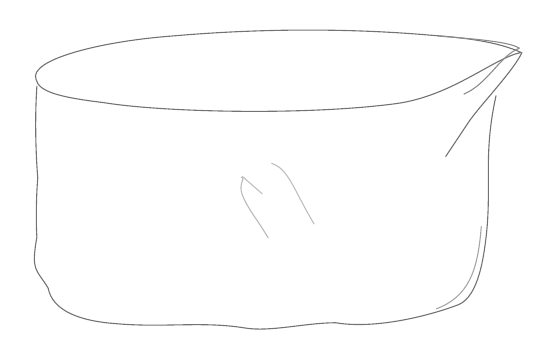
\begin{tikzpicture}[x=.011cm,y=-.011cm,line cap=round,line join=round]
\draw[black!55,thin] (8,66) .. controls (-1,43) and (84,22) .. (165,16)
 .. controls (268,7) and (370,7) .. (463,15)
 .. controls (505,18) and (542,23) .. (568,35)
 .. controls (537,41) and (489,85) .. (424,94)
 .. controls (319,108) and (155,104) .. (87,93)
 .. controls (38,87) and (11,81) .. (8,66);
\draw[black!55,thin] (9,74) .. controls (7,103) and (7,142) .. (10,180)
 .. controls (8,203) and (8,235) .. (9,248)
 .. controls (2,288) and (8,284) .. (22,307)
 .. controls (27,333) and (58,345) .. (100,348)
 .. controls (155,353) and (200,345) .. (249,353)
 .. controls (278,358) and (319,347) .. (354,347)
 .. controls (401,355) and (465,338) .. (496,326)
 .. controls (519,316) and (525,271) .. (528,244)
 .. controls (534,187) and (524,153) .. (539,85);
\draw[black!45,thin] (472,16) .. controls (523,20) and (554,23) .. (566,30)
 .. controls (543,39) and (530,71) .. (502,83);
\draw[black!55,thin] (569,35) .. controls (559,56) and (526,90) .. (509,113) -- (481,155);
\draw[black!35,thin] (522,236) .. controls (518,288) and (507,317) .. (470,331);
\draw[black!27,thin] (245,179) .. controls (251,179) and (241,186) .. (246,199)
 .. controls (252,215) and (263,227) .. (276,249);
\draw[black!25,thin] (246,178) -- (269,198);
\draw[black!25,thin] (280,163) .. controls (300,170) and (304,191) .. (329,233);
\end{tikzpicture}}
% archive sheet number: 28

\scanpage{30}
\textbf{C. R. Acad. Sc. Paris, t. 278 (27 mai 1974)}\hfill\textbf{Série A ---}\mspage{1401}\par\noindent\rule{\linewidth}{.35pt}\par

TOPOLOGIE. --- \textit{Classification topologique des plongements des 1-complexes compacts dans les surfaces.} Note (*) de M. \textbf{Yves Ladegaillerie}, présentée par M. Henri Cartan.

{\small On étudie d'abord le cas des surfaces compactes orientées en utilisant une notion d'équivalence de plongements par homéomorphisme. On caractérise alors les classes d'équivalence à l'aide d'invariants.}

1. \textsc{Catégorie des 1-complexes a isotopie près.}

1.1. On appellera \textit{étoile standard} à \(n\) branches (\(n\geqq1\)), la partie de \(\mathbf{R}^2\) définie en coordonnées polaires par \(\{(\rho,\theta),0\leqq\rho\leqq1,\theta=(2\,k\,\pi/n), k\in\mathbf{Z}\}\). On appellera \textit{étoile} tout espace topologique homéomorphe à une étoile standard ou réduit à un point (0 branche). Un \textit{1-complexe compact} est un espace topologique compact dont tout point a un voisinage homéomorphe à une étoile à \(n\) branches; si \(n\ne2\), on dira que c'est un \textit{sommet}, si \(n=0\) c'est un \textit{sommet isolé}.

1.2. On notera \(\mathscr{K}_{\mathscr I}\) la catégorie des \textit{1-complexes à isotopie près}, dont les objets son\textsuperscript{t} les 1-complexes compacts et les morphismes sont les \textit{classes d'isotopie} d'homéomorphismes. On notera \(\mathscr{K}_{\mathscr C}\) la catégorie des \textit{1-complexes combinatoires} dont les objets sont les 5-uples \((\mathrm{S},\mathrm{A},\mathrm{A}_1,\sigma,s)\), où \(\mathrm{S},\mathrm{A},\mathrm{A}_1\) sont des ensembles finis, \(\mathrm{A}_1\subset\mathrm{A}\), \(\sigma\) une involution sans point fixe de \(\mathrm{A}\) telle que \(\sigma(\mathrm{A}_1)=\mathrm{A}_1\), \(s\) une application de \(\mathrm{A}_1\) dans \(\mathrm{S}\) telle qu'il n'existe pas de \(x\) de \(\mathrm{S}\) tel que \(\operatorname{card}(s^{-1}(x))=2\). Un morphisme entre \((\mathrm{S},\mathrm{A},\mathrm{A}_1,\sigma,s)\) et \((\mathrm{S}',\mathrm{A}',\mathrm{A}'_1,\sigma',s')\) est un couple \((\varphi,\psi)\), où \(\varphi\) est une bijection de \(\mathrm{S}\) sur \(\mathrm{S}'\), \(\psi\) une bijection de \(\mathrm{A}\) sur \(\mathrm{A}'\) telles que \(\psi(\mathrm{A}_1)=\mathrm{A}'_1\), \(\varphi\circ s=s'\circ\psi\vert_{\mathrm{A}_1}\), \(\psi\circ\sigma=\sigma'\circ\psi\).

1.3. On définit un foncteur \(\mathscr{C}\) de \(\mathscr{K}_{\mathscr I}\) dans \(\mathscr{K}_{\mathscr C}\) en associant au 1-complexe \(\mathrm{K}\) le 5-uple \((\mathrm{S},\mathrm{A},\mathrm{A}_1,\sigma,s)\), où \(\mathrm{S}\) est l'ensemble (fini) des sommets de \(\mathrm{K}\), \(\mathrm{A}\) l'ensemble (fini) des \textit{arcs} de \(\mathrm{K}\) (un arc étant une arête orientée et une arête une composante connexe de \(\mathrm{K}\setminus\mathrm{S}\)), \(\mathrm{A}_1\) l'ensemble des arcs ayant une source, \(s\) l'application de \(\mathrm{A}_1\) dans \(\mathrm{S}\) qui à un tel arc associe sa source, \(\sigma\) l'involution de \(\mathrm{A}\) qui a un arc associe son inverse.

1.4. \textsc{Théorème.} --- \textit{Le foncteur \(\mathscr{C}\) est une équivalence de catégories.}

2. \textsc{Préliminaires topologiques.} --- \textit{Terminologie.} --- Une surface (resp. surface à bord) est une 2-variété topologique (resp. 2-variété à bord).

2.1. On appellera \textit{plongement} d'un 1-complexe \(\mathrm{K}\) dans une surface à bord orientée \(\mathrm{V}\) : une injection continue de \(\mathrm{K}\) dans l'intérieur de \(\mathrm{V}\).

2.2. \textsc{Proposition.} --- \textit{Toute injection continue de \([0,1]\) dans \(\mathbf{R}^2\) se prolonge en un homéomorphisme de \(\mathbf{R}^2\) sur lui-même} [\textit{voir} (\textsuperscript{2}), (\textsuperscript{3}), (\textsuperscript{4})].

2.3. \textsc{Proposition.} --- \textit{Tout plongement d'une étoile \(\mathrm{K}\) dans \(\mathbf{R}^2\) orienté détermine de façon canonique un ordre circulaire sur l'ensemble des branches de \(\mathrm{K}\) et est isotope par isotopie ambiante à un plongement standard} (1.1) \textit{induisant le même ordre circulaire.}

2.4. \textsc{Définition.} --- Deux plongements \(f_1\) et \(f_2\) d'un 1-complexe compact \(\mathrm{K}\) dans deux surfaces orientées à bords \(\mathrm{V}_1\) et \(\mathrm{V}_2\) sont dits \textit{équivalents} s'il existe un homéomorphisme orienté \(h\) de \(\mathrm{V}_1\) sur \(\mathrm{V}_2\) tel que \(h\circ f_1=f_2\).
% archive sheet number: 29

\scanpage{31}
\mspage{1402}\textbf{--- Série A}\hfill\textbf{C. R. Acad. Sc. Paris, t. 278 (27 mai 1974)}\par\noindent\rule{\linewidth}{.35pt}\par

2.5. \textsc{Proposition.} --- \textit{Soient \(\mathrm{W},\mathrm{W}'\) deux surfaces à bords \(\partial\mathrm{W},\partial\mathrm{W}'\) orientées et de même genre (nombre d'anses), et \(h\) un homéomorphisme orienté de \(\partial\mathrm{W}\) sur \(\partial\mathrm{W}'\); alors \(h\) s'étend en un homéomorphisme orienté de \(\mathrm{W}\) sur \(\mathrm{W}'\).}

3. \textsc{Voisinage tubulaire standard d'un 1-complexe circularisé.} --- Dans la suite, \(\mathrm{K}\) désigne un 1-complexe compact.

3.1. On appellera \textit{1-complexe circularisé} le couple \((\mathrm{K},\omega)\) fermé de \(\mathrm{K}\) et d'une famille (circularisation) \(\omega=(\omega_x)_{x\in\mathrm{S}}\), où pour tout sommet \(x\in\mathrm{S}\), \(\omega_x\) est un ordre circulaire sur l'ensemble des arcs issus de \(x\). [Cette notion a d'abord été systématisée dans le contexte combinatoire dans (\textsuperscript{1}).]

3.2. A tout 1-complexe circularisé \((\mathrm{K},\omega)\) est associé son \textit{voisinage tubulaire standard} \(\mathrm{T}(\mathrm{K},\omega)\) qui est une surface à bord orientée obtenue par réunion et recollement de la façon suivante : à tout sommet isolé \(x\) on associe un disque orienté \(\mathrm{D}_x\); à tout arc \(a\in\mathrm{A}\) on associe le rectangle \(\bar a\times\mathrm{I}\) (où \(\mathrm{I}=[-1,+1]\)) avec l'orientation produit; (\(\bar a\) est l'arc compactifié par 2 extrémités); on identifie les points de \(\bar a\times\mathrm{I}\) et de \(\overline{\sigma(a)}\times\mathrm{I}\) selon la loi \((p,t)\sim(p,-t)\). Pour tout arc \(a\) ayant une source \(x\in\mathrm{S}\), on considère \(a'=\omega_x(a)\) et on recolle les rectangles orientés \(\bar a\times\mathrm{I}\) et \(\bar a'\times\mathrm{I}\) en identifiant les points \((x,t)\) et \((x,-t)\) pour \(t\in[0,1]\).

3.3. On a un plongement canonique \(i_\omega\) de \(\mathrm{K}\) dans \(\mathrm{T}(\mathrm{K},\omega)\), induit par le plongement canonique \((p\to(p,0))\) de \(\bar a\) dans \(\bar a\times\mathrm{I}\), un sommet isolé \(x\) étant envoyé sur le centre du disque \(\mathrm{D}_x\) associé. Le plongement \(i_\omega\) est caractérisé à équivalence près (2.4) par la propriété d'être une équivalence d'homotopie.

3.4. Soit \((\mathrm{K},\omega)\) un 1-complexe circularisé et \(\mathrm{E}\) l'ensemble des arcs et des sommets isolés \(\mathrm{K}\). On définit une permutation \(\varphi_\omega\) de \(\mathrm{E}\) de la manière suivante : soit \(a\) un arc ayant une source, soit \(x\) son but, on pose \(\varphi_\omega(a)=\omega_x(-a)\). Sur les autres éléments de \(\mathrm{E}\), \(\varphi_\omega\) est l'identité. Un \(\omega\)-\textit{circuit} de \(\mathrm{K}\) est une orbite de \(\varphi_\omega\). On note \(\mathrm{C}(\mathrm{K},\omega)\) l'ensemble des \(\omega\)-circuits de \(\mathrm{K}\). On définit une bijection canonique entre \(\pi_0(\partial\mathrm{T}(\mathrm{K},\omega))\) et \(\mathrm{C}(\mathrm{K},\omega)\).

4. \textsc{Voisinage tubulaire d'un plongement.}

4.1. \textsc{Théorème.} --- \textit{Étant donné un plongement \(f\) de \(\mathrm{K}\) dans une surface orientée \(\mathrm{V}\), il existe une unique circularisation \(\omega(f)\) de \(\mathrm{K}\) telle qu'il existe une surface à bord \(\mathrm{T}(\mathrm{K},f,\mathrm{V})\) contenue dans \(\mathrm{V}\) (appelée \textup{voisinage tubulaire de} \(f\)), l'intérieur de \(\mathrm{T}(\mathrm{K},f,\mathrm{V})\) contenant \(f(\mathrm{K})\) et telle que le plongement \(f\) de \(\mathrm{K}\) dans \(\mathrm{T}(\mathrm{K},f,\mathrm{V})\) soit équivalent au plongement canonique de \(\mathrm{K}\) dans \(\mathrm{T}(\mathrm{K},\omega(f))\). Il existe alors une bijection canonique \(\psi_f\) entre \(\pi_0(\partial\mathrm{T}(\mathrm{K},f,\mathrm{V}))\) et \(\mathrm{C}(\mathrm{K},\omega(f))\),} (3.4).

4.2. \textsc{Corollaire.} --- \textit{Soit \(f_1\) (resp. \(f_2\)) un plongement de \(\mathrm{K}\) dans \(\mathrm{V}_1\) (resp. \(\mathrm{V}_2\)); on a \(\omega(f_1)=\omega(f_2)\) si et seulement si il existe des voisinages \(\mathrm{T}_1\) et \(\mathrm{T}_2\) de \(f_1(\mathrm{K})\) et \(f_2(\mathrm{K})\) tels que les plongements induits \(g_1\) de \(\mathrm{K}\) dans \(\mathrm{T}_1\) et \(g_2\) de \(\mathrm{K}\) dans \(\mathrm{T}_2\) soient équivalents.}

5. \textsc{Théorème de classification.}

5.1. Si \(f\) est un plongement de \(\mathrm{K}\) dans la surface orientée compacte \(\mathrm{V}\), tel que \(\pi_0(f)\) soit surjectif, \(\mathrm{T}\) un voisinage tubulaire, soit \(\mathrm{V}'=\mathrm{V}\setminus\operatorname{int}\mathrm{T}\); alors \(\mathrm{V}'\) est une surface compacte orientée à bord \(\partial\mathrm{V}'=-\partial\mathrm{T}\). On construit une partition de \(\pi_0(\partial\mathrm{V}')\) en rangeant dans une même classe les éléments contenus dans une même composante connexe de \(\mathrm{V}'\). A cette classe on associe un entier positif ou nul : le genre de cette composante.
% archive sheet number: 30

\scanpage{32}
\textbf{C. R. Acad. Sc. Paris, t. 278 (27 mai 1974)}\hfill\textbf{Série A ---}\mspage{1403}\par\noindent\rule{\linewidth}{.35pt}\par

Par la bijection \(\psi_f\) (4.1), on en déduit une partition \((\mathrm{E}_i)_{i\in\mathrm{I}}\) de \(\mathrm{C}(\mathrm{K},\omega(f))\) et à chaque \(\mathrm{E}_i\) est associé un entier \(n_i\geqq0\). Alors \(\omega(f)\) et la famille \(((\mathrm{E}_i,n_i))_{i\in\mathrm{I}}\) sont des invariants, c'est-à-dire sont inchangés lorsqu'on remplace \(f\) par un plongement équivalent. On les appellera \textit{invariants} du plongement \(f\).

5.2. \textsc{Théorème de classification.} --- \textit{Deux plongements \(f\) et \(f'\) sont équivalents si et seulement s'ils ont mêmes invariants. De plus, tout système d'invariants sur \(\mathrm{K}\) : \(\omega,\ (\mathrm{E}_i,n_i)_{i\in\mathrm{I}}\) provient d'une classe de plongements.}

{\small (*) Séance du 17 avril 1974.

(\textsuperscript{1}) J. R. \textsc{Edmonds}, \textit{A combinatorial representation for polyhedral surfaces} (\textit{Not. A. M. S.}, 7, 1960, p. 646).

(\textsuperscript{2}) J. F. P. \textsc{Hudson}, \textit{Piece-Wise Linear Topology}, W. A. Benjamin Inc., 1969.

(\textsuperscript{3}) R. L. \textsc{Wilder}, \textit{Topology of Manifolds} (\textit{A. M. S.}, Coll. Publ., 32, 1949).

(\textsuperscript{4}) E. C. \textsc{Zeeman}, \textit{Seminar on Combinatorial topology}, I. H. E. S., 1963, Exp. I à VIII.}

\begin{flushright}
\textit{Université des Sciences et Techniques}\\
\textit{du Languedoc,}\\
\textit{Mathématiques,}\\
\textit{Place Eugène-Bataillon,}\\
34000 \textit{Montpellier.}
\end{flushright}
% archive sheet number: 31

